\RequirePackage{currfile} 

\documentclass[aspectratio=169]{beamer}
\usetheme{Boadilla}
\addtobeamertemplate{navigation symbols}{}{%
    \usebeamerfont{footline}%
    \usebeamercolor[fg]{footline}%
    \hspace{1em}%
    \insertframenumber/\inserttotalframenumber
}
\setbeamertemplate{caption}[numbered]
\usepackage{multirow}
\usepackage{multicol}

% \input{preambule/special_beamer.tex}
\input{preambule/autres_packages.tex}
\input{preambule/macros.tex}

\title[Sinh biểu cảm khuôn mặt dựa trên giọng nói]{\textbf{SINH BIỂU CẢM KHUÔN MẶT DỰA TRÊN GIỌNG NÓI}}

\author{Trần Hoàng Tuấn\inst{1}, Nguyễn Quang Hùng\inst{2}}

\institute[HCMUT]{
\inst{1}%
Học viên thực hiện\\
Khoa học máy tính, đại học Bách Khoa thành phố Hồ Chí Minh
\and
\inst{2}%
Tiến sĩ hướng dẫn khoa học\\
Khoa học máy tính, đại học Bách Khoa thành phố Hồ Chí Minh }
\date{Bảo vệ đề cương luận văn, 01/2021} 

\begin{document}
\begin{frame}
\titlepage 
\end{frame}
\frame{\tableofcontents}

\section{Giới thiệu}\label{sec:intro}
\frame{\tableofcontents[currentsection]}

\begin{frame}{Giới thiệu}
Định nghĩa bài toán
\begin{itemize}
    \item Là một bài toán tạo sinh dữ liệu dạng hình ảnh dựa trên các dạng dữ liệu khác.
    \item Cho trước một vài dữ liệu về gương mặt của một người bất kỳ \textit{(hình ảnh, video ngắn)} và môt đoạn tiếng nói bất kỳ. Tạo sinh hình ảnh người đó đang nói đoạn tiếng nói đã cho một cách chân thực.
\begin{figure}[H]
    \centering
    \includegraphics[width=13cm]{images/intro.png}
    \caption{Ví dụ về mô hình tạo sinh khuôn mặt}
    \label{fig:example}
\end{figure}
\end{itemize}
\end{frame}


\begin{frame}{Giới thiệu}
Lý do chọn đề tài
\begin{itemize}
    \item Là nhu cầu cần thiết trong ngành giải trí, phim ảnh, hoạt hình, giúp giảm chi phí sản xuất phim
    \begin{itemize}
        \item Phần hóa trang có thể được cắt bớt
        \item Phần kĩ xảo có thể được đơn giản hóa
    \end{itemize}
    \item Tạo sinh gương mặt đại diện trong trường hợp người nói không muốn lộ diện
    \item Tạo sinh biên tập viên ảo trong chương trình thời sự, dự báo thời tiết
    \item Giả lập trợ lý ảo có hình dáng con người
\end{itemize}
\end{frame}

\begin{frame}{Giới thiệu}
Thách thức
\begin{itemize}
    \item Đây là một đề tài mới lạ, vấn đề tạo sinh dữ liệu chỉ vừa được bùng nổ từ năm 2014 khi mạng GANs xuất hiện
    \item Tạo sinh dữ liệu cũng là một đề tài khó và phức tạp
    \item Tạo sinh video từ những dạng dữ liệu khác (hình ảnh, âm thanh) càng làm cho bài toán trở nên thách thức hơn
    \item Bài toán cũng yêu cầu sức mạnh tính toán lớn và khối lượng dữ liệu lớn
\end{itemize}
\end{frame}

\begin{frame}{Giới thiệu}
\begin{enumerate}
    \item \textit{Mục tiêu}: Xây dựng mô hình có khả năng tạo sinh hình ảnh khuôn mặt người một cách tự nhiên, chính xác.
    \item \textit{Giới hạn}: Tạo sinh hình ảnh trong vùng mặt người. Dữ liệu mẫu được cung cấp ban đầu phải là hình ảnh rõ ràng của khuôn mặt người và một đoạn âm thanh bất kỳ thu âm tiếng nói.
    \item \textit{Đối tượng}: Các phương pháp mô hình hóa bài toán, học máy, học sâu, mạng GANs và các phương pháp tạo sinh dữ liệu từ mạng GANs, các phương pháp kết hợp đặc trưng hình ảnh, âm thanh để tạo sinh dữ liệu mới.
\end{enumerate}
\end{frame}

\section{Các công trình nghiên cứu có liên quan}\label{sec:related_works}
\frame{\tableofcontents[currentsection]}

\subsection{Mạng GANs}
\begin{frame}{Mạng GANs}
\begin{figure}[H]
    \centering
    \includegraphics[width=12cm]{./images/gans-pure.png}
    \caption{Cấu trúc mạng GANs cơ bản}
    \label{fig:pure-gans}
\end{figure}
\end{frame}

\begin{frame}{Mạng GANs}
\begin{figure}[H]
    \centering
    \includegraphics[width=14cm]{./images/gans-faces.png}
    \caption{Tạo sinh hình ảnh mặt người bằng mạng GANs theo các năm}
    \label{fig:gans-faces}
\end{figure}
\end{frame}

\subsection{Tổng quan tình hình nghiên cứu}
\begin{frame}{Tổng quan tình hình nghiên cứu}
\begin{figure}[H]
    \centering
    \includegraphics[width=12.5cm]{images/related_work_tree.png}
    \caption{Tổng quan tình hình nghiên cứu}
    \label{fig:related_work_tree}
\end{figure}
\end{frame}

\subsection{Nghiên cứu Hierarchical Cross-Modal Talking Face Generation With Dynamic Pixel-Wise Loss \cite{chen2019}}

\begin{frame}{Nghiên cứu Hierarchical Cross-Modal Talking Face Generation With Dynamic Pixel-Wise Loss \cite{chen2019}}
    \begin{figure}[H]
    \centering
    \includegraphics[width=10cm]{images/processing-training.png}
    \label{fig:processing-training}
    \caption{Phương thức tạo sinh hình ảnh}
    \end{figure}
\end{frame}

\begin{frame}{Nghiên cứu Hierarchical Cross-Modal Talking Face Generation With Dynamic Pixel-Wise Loss \cite{chen2019}}
    \begin{figure}[H]
    \centering
    \includegraphics[width=12cm]{images/idea-small.png}
    \label{fig:idea}
    \caption{Ý tưởng tạo sinh hình ảnh từ ảnh gốc}
    \end{figure}
\end{frame}

\begin{frame}{Nghiên cứu Hierarchical Cross-Modal Talking Face Generation With Dynamic Pixel-Wise Loss \cite{chen2019}}
Hệ thống gồm có hai thành phần chính:
\begin{itemize}
    \item Mạng dự đoán cột mốc gương mặt ($\Psi$)
    \item Hệ thống mạng GANs:
    \begin{itemize}
        \item Mạng tạo sinh video ($G$)
        \item Mạng phân biệt ($D$)
    \end{itemize}
\end{itemize}
\end{frame}

\begin{frame}{Nghiên cứu Hierarchical Cross-Modal Talking Face Generation With Dynamic Pixel-Wise Loss \cite{chen2019}}
    \begin{figure}[H]
    \centering
    \includegraphics[width=9.5cm]{images/processing-landmark_dec.png}
    \label{fig:processing-landmark_dec}
    \caption{Mạng dự đoán cột mốc gương mặt}
    \end{figure}
\end{frame}

\begin{frame}{Nghiên cứu Hierarchical Cross-Modal Talking Face Generation With Dynamic Pixel-Wise Loss \cite{chen2019}}
    \begin{figure}[H]
    \centering
    \includegraphics[width=9.5cm]{images/processing-gan.png}
    \label{fig:processing-gan}
    \caption{Mạng GANs}
    \end{figure}
\end{frame}

\begin{frame}{Cấu trúc bộ dự đoán cột mốc gương mặt (Landmark Decoder)}
    \begin{figure}[H]
        \centering
        \includegraphics[width=13cm]{images/landmark_decoder.png}
        \label{fig:landmark_decoder}
        \caption{Cấu trúc bộ dự đoán cột mốc gương mặt (Landmark Decoder)}
    \end{figure}
\end{frame}

\begin{frame}{Cấu trúc bộ tạo sinh hình ảnh (Generator)}
    \begin{figure}[H]
        \centering
        \includegraphics[width=10.5cm]{images/generator.png}
        \label{fig:generator}
        \caption{Cấu trúc bộ tạo sinh hình ảnh (Generator)}
    \end{figure}
\end{frame}

\begin{frame}{Cấu trúc bộ phân biệt (Discriminator)}
    \begin{figure}[H]
        \centering
        \includegraphics[width=10cm]{images/discriminator.png}
        \label{fig:discriminator}
        \caption{Cấu trúc bộ phân biệt (Discriminator)}
    \end{figure}
\end{frame}

\begin{frame}{Hàm mất mát tổng}
    \begin{equation}
        \begin{split}
        \mathcal{L}_{gans} = &\mathcal{L}_{gans-dis} + \mathcal{L}_{gans-landmark}\\
        \mathcal{L} = &\mathcal{L}_{gans} + \lambda*\mathcal{L}_{pix}
        \end{split}
    \end{equation}
    Bằng thực nghiệm ta chọn $\lambda = 10$ để cân bằng giữa $\mathcal{L}_{gans}$ và $\mathcal{L}_{pix}$
\end{frame}

\begin{frame}{Hàm mất mát cho từng pixel}
    \begin{equation}
        \mathcal{L}_{pix} = \frac{1}{T}\sum^T_{t=1}||(i_{video}(t)-p_{image}(t))*(p_{att}(t)+\beta)||_1
    \end{equation}
    
    Trong đó:
    \begin{itemize}
        \item \textbf{$i_{video}(t)$}: khung hình tại thời điểm $t$ của video gốc
        \item \textbf{$p_{image}(t)$}: hình ảnh được tạo sinh tại thời điểm $t$
        \item \textbf{$p_{att}(t)$}: mặt nạ chú ý được dự đoán tại thời điểm $t$
        \item \textbf{$\beta$}: một hằng số để đảm bảo tất cả các điểm trên ảnh đều được học, bằng thực nghiệm ta chọn $\beta = 0.5$ 
    \end{itemize}
    
\end{frame}

\begin{frame}{Hàm mất mát GANs cho bộ phân biệt}
    \begin{equation}
        \begin{split}
        \mathcal{L}_{gans-dis} = &\mathbb{E}_{l_{input},i_{video}}[logD_s(l_{input},i_{video})]\\
        +&\mathbb{E}_{l_{input},i_{input},p_{landmark}}[log(1-D_s(l_{input},G(l_{input},i_{input},p_{landmark})))]
        \end{split}
    \end{equation}
    Trong đó:
    \begin{itemize}
        \item \textbf{$l_{input},i_{input},p_{landmark},i_{video}$}: đã được giải thích ở các phần trên
        \item \textbf{$D_s$}: Mạng phân biệt với đầu ra là xác suất ảnh là ảnh thật
        \item \textbf{$G$}: Mạng tạo sinh hình ảnh
    \end{itemize}
\end{frame}

\begin{frame}{Hàm mất mát GANs cho bộ phân biệt}
\begin{equation}
    \begin{split}
    \mathcal{L}_{gans-landmark} = &||(D_l(l_{input},G(l_{input},i_{input},p_{landmark})) - l_{orig})*M_l||^2_2\\
    +&||(D_l(l_{input},i_{video}) - l_{orig})*M_l||^2_2\\
    \end{split}
\end{equation}

    Trong đó:
    \begin{itemize}
        \item \textbf{$l_{input},i_{input},p_{landmark},i_{video}$}: đã được giải thích ở các phần trên
        \item \textbf{$D_l$}: Mạng phân biệt với đầu ra là cột mốc gương mặt trên ảnh được tạo sinh
        \item \textbf{$G$}: Mạng tạo sinh hình ảnh
        \item \textbf{$l_{original}$}: Cột mốc gương mặt được trích xuất nguyên gốc từ video $i_{video}$
        \item \textbf{$M_l$}: mặt nạ nhằm chú ý nhiều hơn vào cột mốc gương mặt vùng miệng, theo đó, sai số của cột mốc ở vùng miệng có hệ số 100, trong khi các vùng khác là 1.
    \end{itemize}
\end{frame}

\begin{frame}{Tiền xử lý dữ liệu}
    Dữ liệu huấn luyện là các video với mặt người đang nói.
    \begin{itemize}
        \item Âm thanh: được lấy mẫu ở tần số thấp hơn và trích xuất đặc trưng MFCC trước khi đưa vào mạng tạo sinh cột mốc
        \item Hình ảnh: trích xuất và chuẩn hóa hình ảnh gương mặt sao cho mắt, mũi và miệng người nói trong các video có vị trí gần như nhau
        \item Cột mốc gương mặt: trích xuất và chuẩn hóa cột mốc gương mặt từ các video sao cho tất cả các cột mốc gương mặt đều đồng nhất với nhau
    \end{itemize}
\end{frame}

\section{Phương pháp đề xuất}\label{sec:method}
\frame{\tableofcontents[currentsection]}

\subsection{Ý tưởng thực hiện luận văn}
\begin{frame}{Ý tưởng thực hiện luận văn}
    \begin{itemize}
        \item Luận văn kế thừa kết quả nghiên cứu của Lele Chen và cộng sự \cite{chen2019}
        \begin{itemize}
            \item Nắm rõ ý tưởng của tác giả và quy trình công nghệ
            \item Thực nghiệm lại mô hình tạo sinh hình ảnh của tác giả
        \end{itemize}
        \item Luận văn cũng kết hợp có chỉnh sửa cách chuẩn hóa cột mốc gương mặt từ nghiên cứu Generating Talking Face Landmarks from Speech\cite{gen_face_landmark} để cho kết quả tạo sinh tốt hơn
        \begin{itemize}
            \item Cột mốc gương mặt phải có cùng kích thước
            \item Vị trí của mắt, mũi, miệng trên cột mốc gương mặt cần phải được chuyển về một vị trí đồng nhất cho mọi khung hình
            \item Hạn chế việc ảnh hưởng của đặc điểm nhận dạng của khuôn mặt lên cột mốc gương mặt
        \end{itemize}
    \end{itemize}
\end{frame}

\begin{frame}{Ý tưởng thực hiện luận văn}
    \begin{figure}[H]
        \centering
        \includegraphics[width=9.5cm]{images/processing-contrib.png}
        \label{fig:processing-contrib}
        \caption{Chuẩn hóa cột mốc gương mặt trước khi đưa vào mạng}
    \end{figure}
\end{frame}

\subsection{Tiền xử lý dữ liệu}
\begin{frame}{Tiền xử lý dữ liệu}
    Ta mong muốn đầu vào của mạng là một cột mốc gương mặt chung nhất và không bị ảnh hưởng bởi đặc điểm mặt người trên video. Vì vậy, ta cần tạo ra cột mốc gương mặt chuẩn bằng cách lấy trung bình cộng của nhiều cột mốc trong nhiều video khác nhau
    \begin{figure}[H]
        \centering
        \includegraphics[width=6cm]{images/standard_landmark.png}
        \label{fig:standard_landmark}
        \caption{Cột mốc gương mặt chuẩn}
    \end{figure}
\end{frame}

\begin{frame}{Tiền xử lý dữ liệu}
    Ý tưởng chuẩn hóa cột mốc gương mặt
    \begin{itemize}
        \item Chuyển vùng mắt của cột mốc gương mặt trong video về vị trí tương ứng trên cột mốc chuẩn
        \item Tìm đạo hàm của chuỗi cột mốc gương mặt, tính tổng cộng dồn của đạo hàm này để tìm ra sự thay đổi của cột mốc tại thời điểm $t$ so với thời điểm ban đầu
        \item Chuyển sự thay đổi này lên cột mốc gương mặt chuẩn
        \item Điều chỉnh lại vùng mũi, miệng của cột mốc gương mặt vừa được tính toán ra bằng các phép biến đổi Affine để khớp hơn với cột mốc chuẩn
    \end{itemize}
\end{frame}

\begin{frame}{Tiền xử lý dữ liệu}
    Với cách chuẩn hóa nêu trên, ta có thể đưa chuyển động của cột mốc gương mặt ban đầu lên cột mốc gương mặt chuẩn, với các góc độ quay khác nhau của video và loại bỏ đặc điểm gương mặt người nói
    \begin{figure}[H]
        \centering
        \includegraphics[width=11cm]{images/standardized_landmark.png}
        \label{fig:standardized_landmark}
        \caption{Kết quả chuẩn hóa cột mốc gương mặt. Cột mốc ban đầu (xanh), chuẩn hóa (đỏ)}
    \end{figure}
\end{frame}

\begin{frame}{Tiền xử lý dữ liệu}
    Nhờ việc điểu chỉnh lại cột mốc gương mặt ở vùng mũi và miệng, vùng miệng của gương mặt được đưa về gần nhất với vùng miệng của cột mốc chuẩn, vì vậy tất cả các cột mốc được tính toán sẽ có cùng một kích thước vùng miệng, giúp cho mạng dễ học hơn
    \begin{figure}[H]
        \centering
        \includegraphics[width=11cm]{images/landmark_alignment.png}
        \label{fig:landmark_alignment}
        \caption{Kết quả chuẩn hóa vùng miệng. Cột mốc chưa chuẩn hóa (xanh), chuẩn hóa (đỏ)}
    \end{figure}
\end{frame}

\begin{frame}{Tiền xử lý dữ liệu}
    Dựa vào cột mốc gương mặt được trích xuất và chuẩn hóa, ta cũng sử dụng phép biến đổi Affine trên các khung hình trong video, để đưa gương mặt trên hình về vị trí khớp nhất với cột mốc chuẩn
    \begin{figure}[H]
        \centering
        \includegraphics[width=9cm]{images/preprocessed-image.png}
        \label{fig:preprocessed-image}
        \caption{Kết quả chuẩn hóa hình ảnh}
    \end{figure}
\end{frame}

\subsection{Các tập dữ liệu được sử dụng}
\begin{frame}{Các tập dữ liệu được sử dụng}
Tập dữ liệu GRID: Tập dữ liệu chứa 1000 câu, được nói bởi 34 người khác nhau. Như vậy, tập dữ liệu này chứa 34000 video với chất lượng cao, mỗi video có độ dài 3 giây.

    \begin{figure}[H]
        \centering
        \includegraphics[width=7cm]{./images/grid.png}
        \caption{Ảnh trích xuất từ các video trong tập dữ liệu GRID}
    \end{figure}
\end{frame}

\begin{frame}{Các tập dữ liệu được sử dụng}
Tập dữ liệu LRW: Tập dữ liệu chứa hơn 1 triệu video khác nhau, mỗi video có độ dài 1.16 giây, gồm 29 khung hình. Những video này được chia làm 1000 từ vựng, mỗi từ vựng được nói bởi hơn 1000 người khác nhau. Tổng cộng, tập dữ liệu LRW chứa gần 1000 giờ video.
    \begin{figure}[H]
        \centering
        \includegraphics[width=5cm]{./images/lrw.png}
        \caption{Ảnh trích xuất từ các video trong tập dữ liệu LRW}
    \end{figure}
\end{frame}

\subsection{Các độ đo được sử dụng}
\begin{frame}{Các độ đo được sử dụng}
Độ đo SSIM: Là độ đo sự tương đồng về mặt cảm quan giữa hai hình ảnh, dựa trên ba yếu tố là độ tương phản, ánh sáng, và cấu trúc của ảnh. Càng gần về 1, ảnh tạo sinh càng giống với ảnh gốc.
\begin{equation}
SSIM(x,y) = \frac{(2\mu_x\mu_y + C_1) + (2 \sigma _{xy} + C_2)} 
    {(\mu_x^2 + \mu_y^2+C_1) (\sigma_x^2 + \sigma_y^2+C_2)}
\label{eq:SSMI}
\end{equation}
Với:
\begin{itemize}
    \item $\mu_x$, $\mu_y$: trung bình của các điểm ảnh trong cửa sổ
    \item $\sigma_x^2$, $\sigma_y^2$: variance của các điểm ảnh trong cửa sổ
    \item $C_1$, $C_2$: hằng số để ổn định phép chia
\end{itemize}
\end{frame}

\begin{frame}{Các độ đo được sử dụng}
Độ đo CPBD: Là độ đo thể hiện sự sắc nét của hình ảnh, là xác suất tích lũy của các cạnh trên ảnh nếu không được xem là cạnh mờ (blur). Một cạnh được xem là mờ khi nó có độ dày quá lớn, vượt qua độ dày được quy định là mờ $W_{JNB}$
\begin{equation}
CPBD = P(P_{BLUR} < P_{JNB}) = \sum^{P_{BLUR} = P_{JNB}}_{P_{BLUR} = 0}(P_{BLUR})
\label{eq:CPBD}
\end{equation}
Với:
\begin{itemize}
    \item $P_{BLUR}$: xác suất một cạnh bị mờ. $P_{BLUR} = 1 - e^{-(\frac{W_{e(i)}}{W_{JNB}(e_i)})^\beta}$
    \item $W_{JNB}$: Độ dày cạnh quy định là mờ
    \begin{itemize}
        \item $W_{JNB} = 5$ nếu độ tương phản nhỏ hơn hoặc bằng 50
        \item  $W_{JNB} = 3$ nếu độ tương phản lớn hơn 50
    \end{itemize}
\end{itemize}
\end{frame}

\subsection{Môi trường thí nghiệm}
\begin{frame}{Môi trường thí nghiệm}
\begin{table}[h]
    \centering
    \begin{tabular}{c | c | c}
    \hline 
    &\textbf{Máy A} & \textbf{Máy B}\\
    \hline
    \textbf{CPU} & Intel Xeon & Intel Core I5 8600K\\
    \textbf{Bộ nhớ} & 24GB & 32GB\\
    \textbf{GPU} & NVIDIA TESLA V100 & NVIDIA Geforce RTX 3070\\
    \textbf{Ổ cứng} & 160GB SSD & 768GB NVME SSD + 2TB HDD\\
    \textbf{OS} & N/A(Colab Pro) & Ubuntu 20.04\\
    \textbf{Ngôn ngữ} & Python 3.7 & Python 3.7\\
    \textbf{Framework} & Pytorch 1.8 & Pytorch 1.8\\
    \hline
    \end{tabular}
    \caption{Các môi trường được sử dụng trong việc tiền xử lý dữ liệu, huấn luyện và thực hiện thí nghiệm}
    \label{table:hardware}
\end{table}
\end{frame}

\subsection{Thực hiện thí nghiệm}
\begin{frame}{Thực hiện thí nghiệm}
Quá trình huấn luyện mạng tạo sinh cột mốc gương mặt:
\begin{table}[h]
    \centering
    \begin{tabular}{c | c | c}
    \hline 
    &\textbf{GRID} & \textbf{LRW}\\
    \hline
    \textbf{Bộ tối ưu} & Adam & Adam\\
    \textbf{Kích thước bó} & 100 & 100\\
    \textbf{Hệ số học} & 0.001 & 0.0002\\
    \textbf{Thời gian huấn luyện} & 5 phút & 70 phút\\
    \textbf{$\mathcal{L}_{landmark}$} & $4.9200 \times 10^{-4}$ & $2.012 \times 10^{-4}$\\
    \hline
    \end{tabular}
    \caption{Chi tiết huấn luyện mạng tạo sinh cột mốc gương mặt. Giá trị mất mát (trên tập kiểm thử) và thời gian huấn luyện được ghi nhận tại vòng lặp cho ra mô hình tối ưu}
    \label{table:landmark_decoder_training_detail}
\end{table}
\end{frame}

\begin{frame}{Thực hiện thí nghiệm}
Quá trình huấn luyện mạng GANs:
    \begin{table}[h]
    \centering
    \begin{tabular}{c | c | c}
    \hline 
    &\textbf{GRID} & \textbf{LRW}\\
    \hline
    \textbf{Bộ tối ưu} & Adam & Adam\\
    \textbf{Kích thước bó} & 12 & 17\\
    \textbf{Hệ số học} & 0.0002 & 0.0002\\
    \textbf{Thời gian huấn luyện} & 5 giờ 20 phút & 250 giờ\\
    \textbf{$\mathcal{L}_{pix}$} & $4.1575 \times 10^{-2}$ & $6.8502 \times 10^{-2}$\\
    \textbf{$\mathcal{L}_{gans-dis}$} & $0.9964$ & $0.6931$\\
    \textbf{$\mathcal{L}_{gans-landmark}$} & $7.6990 \times 10^{-2}$ & $5.2412 \times 10^{-2}$\\
    \textbf{$\mathcal{L}$} & $1.4892$ & $1.4306$\\
    \hline
    \end{tabular}
    \caption{Chi tiết huấn luyện mạng GANs. Giá trị mất mát (trên tập kiểm thử) và thời gian huấn luyện được ghi nhận tại vòng lặp cho ra mô hình tối ưu}
    \label{table:gans_training_detail}
\end{table}
\end{frame}


\section{Kết quả thí nghiệm}\label{sec:result}
\frame{\tableofcontents[currentsection]}

\begin{frame}{Kết quả thí nghiệm}
Tạo sinh cột mốc gương mặt trên tập GRID. Cột mốc tạo sinh (đỏ) bám tốt theo cột mốc gốc (xanh)
\begin{figure}[H]
    \centering
    \includegraphics[width=15cm]{images/grid_examples-landmark.png}
    \caption{Kết quả tạo sinh cột mốc gương mặt theo giọng nói trên tập GRID. Cột mốc gốc màu xanh, cột mộc tạo sinh màu đỏ}
\end{figure}
\end{frame}

\begin{frame}{Kết quả thí nghiệm}
Tạo sinh cột mốc gương mặt trên tập LRW. Cột mốc tạo sinh (đỏ) bám tốt theo cột mốc gốc (xanh)
\begin{figure}[H]
    \centering
    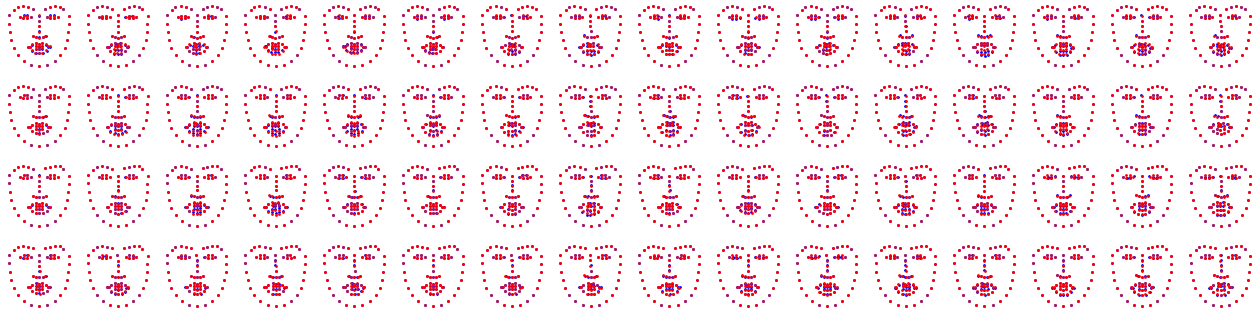
\includegraphics[width=15cm]{images/lrw_examples-landmark.png}
    \caption{Kết quả tạo sinh cột mốc gương mặt theo giọng nói trên tập LRW. Cột mốc gốc màu xanh, cột mộc tạo sinh màu đỏ}
\end{figure}
\end{frame}

\begin{frame}{Kết quả thí nghiệm}
Tạo sinh gương mặt trên tập GRID. Hầu hết video được tạo sinh trên tập test đều rõ ràng, có chuyển động miệng hợp lý
\begin{figure}[H]
    \centering
    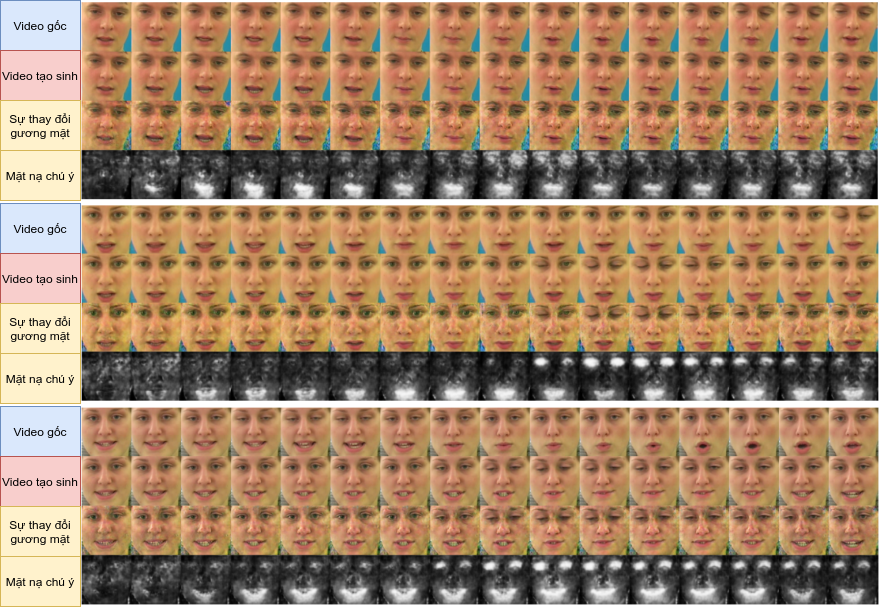
\includegraphics[width=15cm]{images/grid_examples-face.png}
    \caption{Kết quả tạo sinh gương mặt theo giọng nói trên tập GRID}
\end{figure}
\end{frame}

\begin{frame}{Kết quả thí nghiệm}
Tạo sinh gương mặt trên tập LRW. Hầu hết video được tạo sinh tốt khi hình ảnh đầu vào là hình chụp thẳng mặt. Chất lượng video bị suy giảm khi hình ảnh đầu vào được chụp ở các góc nghiêng
\begin{figure}[H]
    \centering
    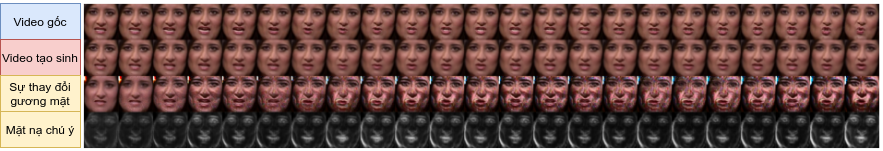
\includegraphics[width=15cm]{images/lrw_examples-face.png}
    \caption{Kết quả tạo sinh gương mặt theo giọng nói trên tập LRW}
\end{figure}
\end{frame}

\begin{frame}{Kết quả thí nghiệm}
\begin{table}[h]
    \centering
    \begin{tabular}{c | c | c | c | c}
    \hline 
    \multirow{2}{*}{\textbf{Phương pháp}} & \multicolumn{2}{c|}{\textbf{GRID}} & \multicolumn{2}{c}{\textbf{LRW}}\\
    \cline{2-5}
    & SSIM & CPBD & SSIM & CPBD\\
    \hline
    \textbf{Zakharov et al \cite{zakharov}} & 0.54 & 0.19 & 0.42 & 0.11 \\
    \textbf{Chung et al \cite{chung}} & 0.41 & \textbf{0.22} & 0.34 & \textbf{0.21} \\
    \textbf{Baseline (Chen et al) \cite{chen2019}} & 0.41 & 0.08 & 0.38 & 0.07 \\
    \hline
    \hline
    \textbf{Ours} & \textbf{0.72} & 0.12 & \textbf{0.54} & 0.06 \\
    \hline
    \end{tabular}
    \caption{So sánh với các mạng có cùng mục tiêu về độ đo SSIM và CPBD. Dữ liệu trong bảng được lấy từ bài khảo sát \cite{chen_survey}}
    \label{table:metrics_result}
\end{table}
Qua bảng trên ta thấy:
\begin{itemize}
    \item Độ tương đồng SSIM đã tăng đáng kể cho cả hai tập dữ liệu. Do đó, video tạo sinh có chuyển động giống video gốc hơn
    \item Độ nét tăng đối với tập GRID, tuy nhiên lại giảm trên tập LRW
\end{itemize}
\end{frame}

\begin{frame}{So sánh với mô hình gốc của Lele Chen}
    \begin{figure}[H]
        \centering
        \includegraphics[width=5cm]{images/comparision-grid.png}
        \caption{So sánh với mô hình của tác giả trên tập GRID. Bên trái là video được tạo sinh bởi mô hình mới, bên phải là của tác giả Lele Chen}
    \end{figure}
\end{frame}

\begin{frame}{So sánh với mô hình gốc của Lele Chen}
    \begin{figure}[H]
        \centering
        \includegraphics[width=10cm]{images/comparision-lrw.png}
        \caption{So sánh với mô hình của tác giả trên tập LRW. Bên trái là video được tạo sinh bởi mô hình mới, bên phải là của tác giả Lele Chen}
    \end{figure}
\end{frame}

\begin{frame}{So sánh với mô hình gốc của Lele Chen}
Về mặt cảm quan, ta thấy
\begin{itemize}
    \item Đối với thử nghiệm trên tập GRID, hình ảnh được tạo sinh bới mô hình mới có độ nét cao hơn
    \item Đối với thử nghiệm trên tập LRW, hình ảnh được tạo sinh bới mô hình mới có độ nét thấp hơn
    \item Trên video thực tế, thử nghiệm trên cả hai tập cho kết quả tạo sinh mượt mà hơn và khẩu hình miệng khớp hơn trên mô hình mới
\end{itemize}
Điều này phù hợp với kết quả khảo sát về độ đo SSIM và CPBD
\end{frame}

\section{Kết luận}\label{sec:conclusion}
\frame{\tableofcontents[currentsection]}
\begin{frame}{Kết luận}
\begin{itemize}
    \item Nghiên cứu đã chạy thử và kiểm chứng lại cấu trúc mạng của Lele Chen và cộng sự \cite{chen2019}
    \item Áp dụng có chỉnh sửa phương pháp chuẩn hóa cột mốc gương mặt từ bài báo \cite{gen_face_landmark} để cho ra kết quả tạo sinh hình ảnh tốt hơn so với bài báo gốc
    \item So sánh với các nghiên cứu mới, kết quả tạo sinh ảnh của của mô hình vẫn còn kém hơn
    \item Tuy nhiên các nghiên cứu có kết quả tốt đòi hỏi quá nhiều tài nguyên tính toán, và khó có thể hiện thực trong điều kiện của tác giả
    \item Nghiên cứu có tiềm năng phát triển thêm để tạo thành một phần mềm tạo sinh biên tập viên ảo. Tác giả cũng đã tạo sinh thử hình ảnh của người Việt và âm thanh tiếng Việt
    \item Có thể phát triển thêm theo hướng sử dụng cột mốc gương mặt trong không gian 3 chiều, và tính toán chuyển động của đầu để video chân thực hơn
\end{itemize}
\end{frame}

\bibliographystyle{unsrt}
\bibliography{references}
\include{./references}



\begin{frame}
    \textbf{\LARGE{\begin{center}Thank you for your attention\end{center}}}
\end{frame}

\end{document}
